\chapter{Sprint 2 — Real-Time Collaboration \& AI Core}
\label{chap:sprint2}

\section{Introduction}

Following Sprint 1, which established a functional baseline accessible via a public URL, \textbf{Sprint 2} of the \textbf{MindSpark} platform focuses on transforming the brainstorming workspace into a live, interactive environment enriched by core Artificial Intelligence assistance \cite{backlog}. The primary objective of this iteration is to deliver low-latency, multi-user real-time collaboration—including instant synchronization of ideas, comments, and votes, active user presence indicators, and live participant cursors—alongside structured idea organization through categories, keyword search, multi-criteria filtering, and sorting \cite{backlog}. Furthermore, Sprint 2 expands room governance controls for room creators and introduces foundational generative AI capabilities for topic-based idea generation and idea expansion \cite{backlog}.

To establish a rigorous engineering deliverable, this chapter presents the realization of Sprint 2 across four core pillars:
\begin{enumerate}
    \item \textbf{Sprint Planning and Backlog Governance:} Defining the Sprint 2 goal, delivered business value, and the 21 prioritized user stories across five functional modules \cite{backlog}.
    \item \textbf{Functional Analysis:} Formalizing actor interactions via the Sprint 2 Use Case Diagram and detailed textual use case specifications covering real-time collaboration, idea organization, and AI ideation \cite{backlog}.
    \item \textbf{Architectural and Behavioral Design:} Modeling domain entities, WebSocket services, the \texttt{ai-service} orchestration layer, runtime sequence flows, and room lifecycle state transitions.
    \item \textbf{Implementation, Review, and Retrospective:} Documenting the integrated features, UI verification captures, sprint review validation, and actionable lessons learned for Sprint 3 \cite{backlog}.
\end{enumerate}

Throughout this chapter, technical specifications remain strictly aligned with the verified architecture of the \textbf{MindSpark} codebase—specifically its Java~21 / Spring Boot~4.1.1 backend, Spring WebSocket engine (\texttt{RoomWebSocketHandler}), transaction-bound event listeners, Angular frontend, and multi-tier \texttt{ai-service} microservice \cite{backlog}.

\section{Organisation of Sprint 2}

\subsection{Sprint Goal and Business Value}

The Sprint Goal defined for Sprint 2 is: \emph{``The room feels alive — live updates, cursors, comments, categories and AI idea generation.''} \cite{backlog}

From both an end-user and architectural perspective, this increment delivers five core pillars of value:
\begin{itemize}
    \item \textbf{Real-Time Collaborative Engagement:} Participants immediately observe new ideas, comments, and votes without manual page reloads (\texttt{US-39}), view the active roster of connected participants (\texttt{US-40}), and track other users' cursors moving across the normalized virtual canvas in real time (\texttt{US-41}) \cite{backlog}.
    \item \textbf{Threaded Discussion and Feedback:} Room members can post comments on ideas (\texttt{US-32}), edit or delete their own comments (\texttt{US-33}), and reply directly to existing comments (\texttt{US-34}) to refine concepts collaboratively \cite{backlog}.
    \item \textbf{Structured Idea Organization and Discovery:} Users can organize sticky notes into color-coded categories (\texttt{US-27}), create, rename, and delete categories within a room (\texttt{US-28}), search ideas by keyword (\texttt{US-29}), and filter or sort proposals by category, author, and minimum vote threshold (\texttt{US-30}) \cite{backlog}.
    \item \textbf{Room Governance and Lifecycle Control:} Room creators exercise full moderation control to edit room metadata (\texttt{US-13}), inspect the participants list (\texttt{US-14}), remove participants (\texttt{US-15}), close active sessions into a read-only state (\texttt{US-16}), and delete rooms (\texttt{US-17}) \cite{backlog}.
    \item \textbf{AI-Assisted Ideation and Demo Readiness:} A dedicated backend AI wrapper service encapsulates external LLM providers (\texttt{US-42}) to generate starter ideas from a topic (\texttt{US-43}) and elaborate or expand existing ideas (\texttt{US-44}) \cite{backlog}. In addition, users can update their display name and avatar (\texttt{US-5}), while the engineering team can reset the demonstration environment to a deterministic clean state (\texttt{T5}) \cite{backlog}.
\end{itemize}

\subsection{Sprint 2 Backlog}

Sprint 2 comprises \textbf{21 user stories} prioritized according to the MoSCoW methodology (\textit{Must}, \textit{Should}, \textit{Could}), as detailed in Table~\ref{tab:sprint2-backlog}.

\begin{table}[htbp]
\centering
\caption{Sprint 2 Product Backlog — Real-Time Collaboration \& AI Core (21 User Stories)}
\label{tab:sprint2-backlog}
\small
\begin{tabularx}{\textwidth}{@{} l X l l @{}}
\toprule
\textbf{ID} & \textbf{User Story} & \textbf{Module} & \textbf{Priority} \\
\midrule
\texttt{US-38} & As a developer, I can use an authenticated real-time channel per room (enabler). & Real-Time Collaboration & Must \\
\texttt{US-39} & As a client, I can see new ideas, comments and votes live. & Real-Time Collaboration & Must \\
\texttt{US-40} & As a client, I can see who is currently online in the room. & Real-Time Collaboration & Must \\
\texttt{US-41} & As a client, I can see other participants' cursors live. & Real-Time Collaboration & Must \\
\midrule
\texttt{US-32} & As a client, I can comment on an idea. & Comments & Must \\
\texttt{US-33} & As a client, I can edit or delete my own comments. & Comments & Should \\
\texttt{US-34} & As a client, I can reply to a comment. & Comments & Should \\
\midrule
\texttt{US-27} & As a client, I can organise ideas into categories. & Ideas Organisation & Should \\
\texttt{US-28} & As a client, I can create, rename and delete categories in a room. & Ideas Organisation & Should \\
\texttt{US-29} & As a client, I can search ideas by keyword. & Ideas Organisation & Should \\
\texttt{US-30} & As a client, I can filter ideas by category, author and minimum votes, and sort them. & Ideas Organisation & Should \\
\midrule
\texttt{US-13} & As a room creator, I can edit the room details. & Room Management & Should \\
\texttt{US-14} & As a room creator, I can preview the participants list. & Room Management & Should \\
\texttt{US-15} & As a room creator, I can remove a participant. & Room Management & Should \\
\texttt{US-16} & As a room creator, I can close the room. & Room Management & Should \\
\texttt{US-17} & As a room creator, I can delete the room. & Room Management & Could \\
\midrule
\texttt{US-42} & As a developer, I can use a backend AI service wrapping the LLM provider (enabler). & AI Core \& Profile & Must \\
\texttt{US-43} & As a client, I can use AI to generate ideas based on a topic. & AI Core \& Profile & Must \\
\texttt{US-44} & As a client, I can use AI to improve or expand an idea. & AI Core \& Profile & Must \\
\texttt{US-5}  & As a client, I can edit my name and avatar. & AI Core \& Profile & Should \\
\texttt{T5}    & As a team, we can reset the demo to a known state. & AI Core \& Profile & Should \\
\bottomrule
\end{tabularx}
\end{table}

\section{Sprint 2 Analysis}

\subsection{Sprint 2 Use Case Diagram}

Figure~\ref{fig:sprint2-usecase} illustrates the Sprint 2 Use Case Diagram. Three actors interact within this scope:
\begin{itemize}
    \item \textbf{Participant:} Manages their profile, posts, edits, deletes, and replies to comments, organizes ideas into categories, performs keyword searches and multi-criteria filtering, collaborates in real time (presence, cursors, live board updates), and invokes AI idea generation and expansion \cite{backlog}.
    \item \textbf{Room Creator:} Specializes the \textit{Participant} actor and additionally manages room details, inspects or removes participants, and closes, reopens, or deletes the room \cite{backlog}.
    \item \textbf{AI System (LLM):} Acts as an external secondary actor fulfilling topic-based idea generation and idea expansion requests routed through the backend \texttt{ai-service} wrapper \cite{backlog}.
\end{itemize}

\begin{figure}[htbp]
    \centering
    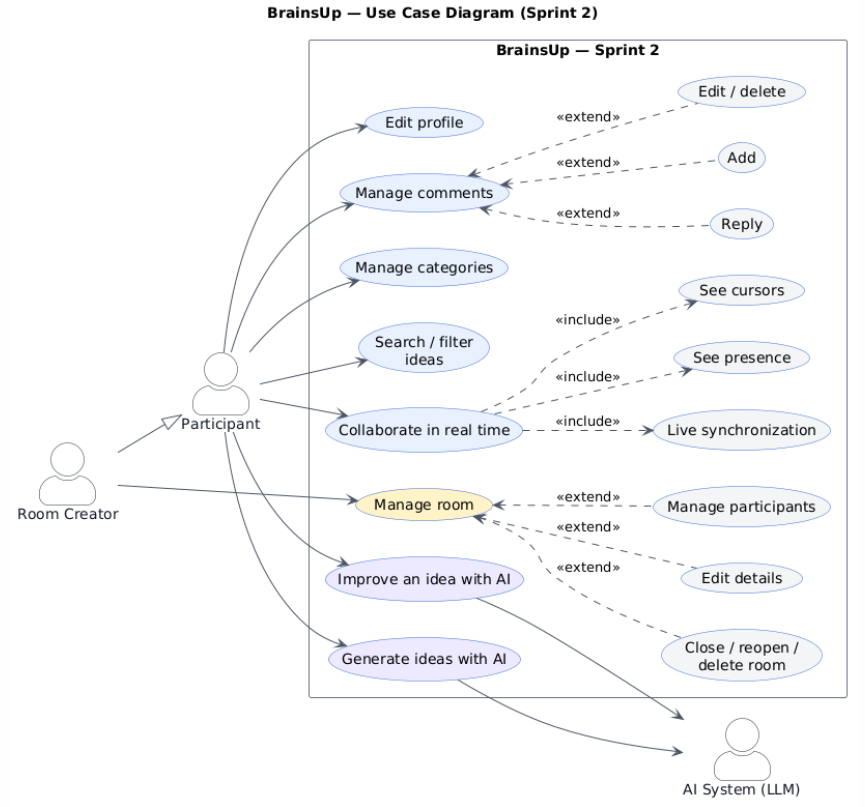
\includegraphics[width=0.88\textwidth]{images/use_case_sprint2.png}
    \caption{Sprint 2 Use Case Diagram covering real-time collaboration, room governance, and AI ideation.}
    \label{fig:sprint2-usecase}
\end{figure}

\subsection{Textual Use Case Descriptions}

To formalize the functional requirements of Sprint 2, Tables~\ref{tab:uc-realtime}, \ref{tab:uc-organise}, and \ref{tab:uc-ai} present the detailed textual specifications of the three primary use case groups.

\begin{table}[htbp]
\centering
\caption{Textual Use Case Description — Real-Time Collaboration in a Room (\texttt{US-38}--\texttt{US-41})}
\label{tab:uc-realtime}
\small
\begin{tabularx}{\textwidth}{@{} l X @{}}
\toprule
\textbf{Attribute} & \textbf{Description} \\
\midrule
\textbf{Use Case} & Collaborate in Real Time in a Room (\texttt{US-38}, \texttt{US-39}, \texttt{US-40}, \texttt{US-41}) \\
\textbf{Actors} & Participant, Room Creator \\
\textbf{Preconditions} & The user holds a valid JWT issued by Keycloak and is an authorized member of the target room. \\
\textbf{Postconditions} & Room mutations (ideas, comments, votes), active presence rosters, and normalized cursor coordinates are synchronized live across all subscribed clients. \\
\textbf{Main Flow} &
1. The participant opens a room workspace, and the Angular client initiates a WebSocket handshake on \texttt{/ws/rooms/\{roomId\}} via the API Gateway (\texttt{US-38}).\newline
2. \texttt{RoomWebSocketHandler} decodes the JWT, verifies room membership through \texttt{RoomService / Auth}, registers a heartbeat in \texttt{PresenceService}, and broadcasts the updated online list (\texttt{US-40}).\newline
3. As the user moves their pointer across the $[0,1000]\times[0,500]$ virtual canvas, throttled cursor coordinates (capped at $25\text{ events/s}$) are emitted and rendered live for peers (\texttt{US-41}).\newline
4. Whenever a participant creates or updates an idea, comment, or vote via the REST API, the committed database transaction triggers \texttt{IdeaChangedEvent} / \texttt{CommentChangedEvent}, broadcasting the update live to all room subscribers (\texttt{US-39}). \\
\textbf{Alternative Flows} &
\textbf{A1 — Invalid Token or Non-Member:} The handler closes the socket with status \texttt{4401} (invalid/expired token) or \texttt{4403} (not a member) and denies access.\newline
\textbf{A2 — Participant Disconnected or Removed:} Upon session closure or removal by the room creator (\texttt{US-15}), \texttt{PresenceService.leave()} evicts the user and broadcasts \texttt{cursor-leave} and updated presence. \\
\bottomrule
\end{tabularx}
\end{table}

\begin{table}[htbp]
\centering
\caption{Textual Use Case Description — Organise, Search, and Filter Ideas (\texttt{US-27}--\texttt{US-30})}
\label{tab:uc-organise}
\small
\begin{tabularx}{\textwidth}{@{} l X @{}}
\toprule
\textbf{Attribute} & \textbf{Description} \\
\midrule
\textbf{Use Case} & Organise, Search, and Filter Ideas (\texttt{US-27}, \texttt{US-28}, \texttt{US-29}, \texttt{US-30}) \\
\textbf{Actors} & Participant, Room Creator \\
\textbf{Preconditions} & The user is authenticated inside an open brainstorming room. \\
\textbf{Postconditions} & Ideas are assigned to thematic categories and rendered according to the active search query, filter predicates, and sort criterion. \\
\textbf{Main Flow} &
1. A participant creates, renames, or deletes categories scoped to the room (\texttt{US-28}) and assigns ideas to categories (\texttt{US-27}).\newline
2. To locate specific proposals, the user enters a search string into the keyword search input (\texttt{US-29}).\newline
3. The user refines the board view by combining filters for category, author, and minimum vote count, and selects a sort order (\texttt{US-30}).\newline
4. The frontend dynamically filters and orders the visible idea cards. \\
\textbf{Alternative Flows} &
\textbf{A1 — Empty Match Set:} If no ideas satisfy the combined keyword and filter predicates, the UI displays an empty-state indicator with a one-click filter reset action. \\
\bottomrule
\end{tabularx}
\end{table}

\begin{table}[htbp]
\centering
\caption{Textual Use Case Description — Generate and Improve or Expand Ideas with AI (\texttt{US-42}--\texttt{US-44})}
\label{tab:uc-ai}
\small
\begin{tabularx}{\textwidth}{@{} l X @{}}
\toprule
\textbf{Attribute} & \textbf{Description} \\
\midrule
\textbf{Use Case} & Generate and Improve or Expand Ideas with AI (\texttt{US-42}, \texttt{US-43}, \texttt{US-44}) \\
\textbf{Actors} & Participant, Room Creator, AI System (LLM) \\
\textbf{Preconditions} & The user is authenticated in an open room, has available daily quota, and the \texttt{ai-service} microservice is reachable. \\
\textbf{Postconditions} & Schema-validated AI idea suggestions or an expanded version of a selected idea are displayed to the user and optionally persisted to the room. \\
\textbf{Main Flow} &
1. The participant enters a brainstorming topic to generate starter ideas (\texttt{US-43}) or selects an existing idea to improve or expand it (\texttt{US-44}).\newline
2. The client calls \texttt{POST /api/ai/ideas/generate} or \texttt{/improve}, routed via the API Gateway to \texttt{IdeaAIController} and \texttt{AIOrchestrator} (\texttt{US-42}).\newline
3. \texttt{AIOrchestrator} reserves quota via \texttt{QuotaService}, builds a structured prompt, and calls \texttt{ModelRouter} to query the external LLM provider and parse/validate the JSON result.\newline
4. The user previews the returned suggestions and adds selected items to the room via \texttt{POST /api/ideas}, persisting them and broadcasting \texttt{idea:created} through \texttt{RoomWebSocketHandler}. \\
\textbf{Alternative Flows} &
\textbf{A1 — Daily Quota Reached:} \texttt{QuotaService.reserve()} rejects the request and returns \texttt{DailyLimitReached} to the UI.\newline
\textbf{A2 — Provider Error or Invalid Output:} \texttt{ModelRouter} attempts the fallback model/provider; if still unsuccessful, \texttt{AIOrchestrator} refunds the reserved quota and returns an HTTP 503 retry message. \\
\bottomrule
\end{tabularx}
\end{table}

\section{Sprint 2 Design}

\subsection{Sprint 2 Class Diagram}

Figure~\ref{fig:sprint2-class} depicts the Sprint 2 Class Diagram, reflecting the exact domain model and backend service architecture of \textbf{MindSpark}:
\begin{itemize}
    \item \textbf{Core Domain Entities:} \texttt{User} (\texttt{id}, \texttt{keycloakId}, \texttt{username}, \texttt{email}, \texttt{dateCreatedAt}) owns and joins \texttt{Room} instances (\texttt{id}, \texttt{name}, \texttt{invitationCode}, \texttt{closed}, \texttt{createdAt}, \texttt{ownerId}, \texttt{memberUserIds}). Each room contains \texttt{Category} (\texttt{id}, \texttt{title}, \texttt{roomId}) and spatial \texttt{Idea} entities (\texttt{id}, \texttt{title}, \texttt{description}, \texttt{text}, \texttt{x}, \texttt{y}, \texttt{color}, timestamps, \texttt{categoryId}, \texttt{authorId}, \texttt{roomId}). \texttt{Comment} (\texttt{id}, \texttt{content}, timestamps, \texttt{ideaId}, \texttt{authorId}, \texttt{parentCommentId}) supports threaded replies via a self-referential parent association (\texttt{US-34}).
    \item \textbf{Real-Time Services:} \texttt{RoomBroadcastEventListener} listens for committed domain events (\texttt{handleIdeaChanged}, \texttt{handleCommentChanged}) and dispatches payloads through \texttt{RoomWebSocketHandler} (\texttt{authenticateAndJoin}, \texttt{handleCursorMove}, \texttt{handleCursorLeave}, \texttt{broadcastToRoom}), which coordinates session tracking with \texttt{PresenceService} (\texttt{heartbeat}, \texttt{leave}).
    \item \textbf{AI Microservice Components (\texttt{ai-service}):} \texttt{IdeaAIController} exposes \texttt{generate(request)} and \texttt{improve(request)} endpoints, delegating execution to \texttt{AIOrchestrator}, which coordinates usage limits with \texttt{QuotaService} (\texttt{reserve}, \texttt{refund}) and dispatches structured prompts through \texttt{ModelRouter} and the \texttt{LlmClient} interface.
\end{itemize}

\begin{figure}[htbp]
    \centering
    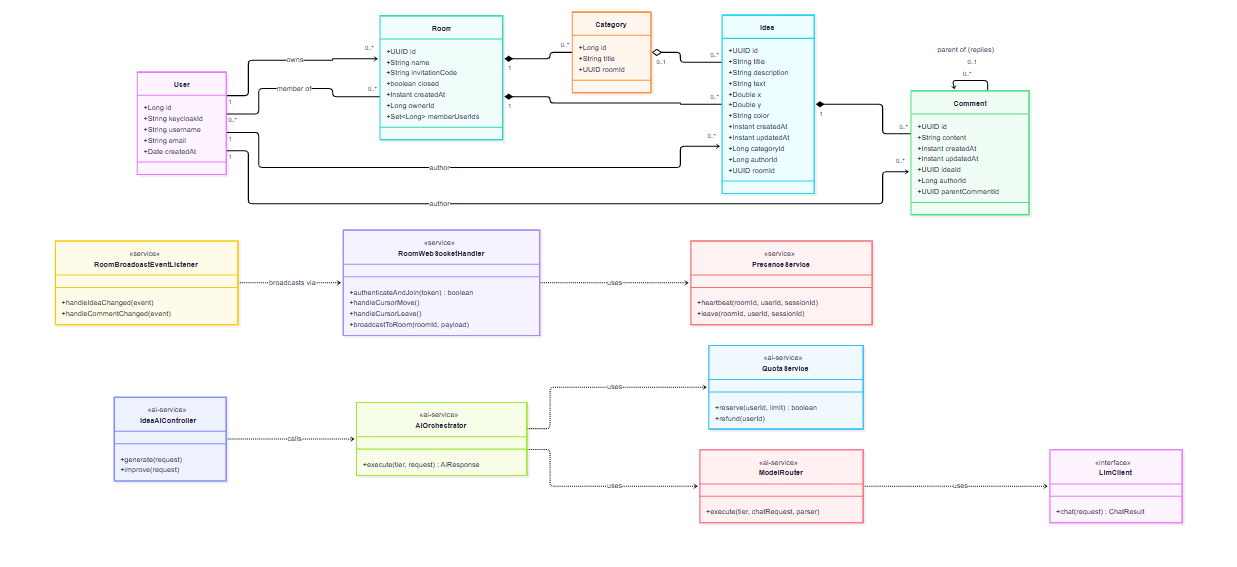
\includegraphics[width=0.98\textwidth]{images/diag_class_sprint2.png}
    \caption{Sprint 2 Class Diagram illustrating domain entities, real-time WebSocket services, and the \texttt{ai-service} orchestration layer.}
    \label{fig:sprint2-class}
\end{figure}

\subsection{Design Sequence Diagrams}

Two sequence diagrams formalize the critical runtime interactions introduced in Sprint 2.

Figure~\ref{fig:sprint2-seq-realtime} illustrates the end-to-end real-time collaboration flow between two participants (\textit{Participant A} and \textit{Participant B}), their frontends, the API Gateway, \texttt{RoomWebSocketHandler}, \texttt{RoomService / Auth}, \texttt{PresenceService}, and the Backend REST API. It models JWT decoding and room membership validation with \texttt{4401}/\texttt{4403} rejection paths (\texttt{US-38}), heartbeat presence registration (\texttt{US-40}), rate-limited cursor broadcasting at $25\text{ events/s}$ (\texttt{US-41}), transaction-safe broadcasting of newly created ideas, comments, and votes (\texttt{US-39}), and clean session disconnection.

\begin{figure}[htbp]
    \centering
    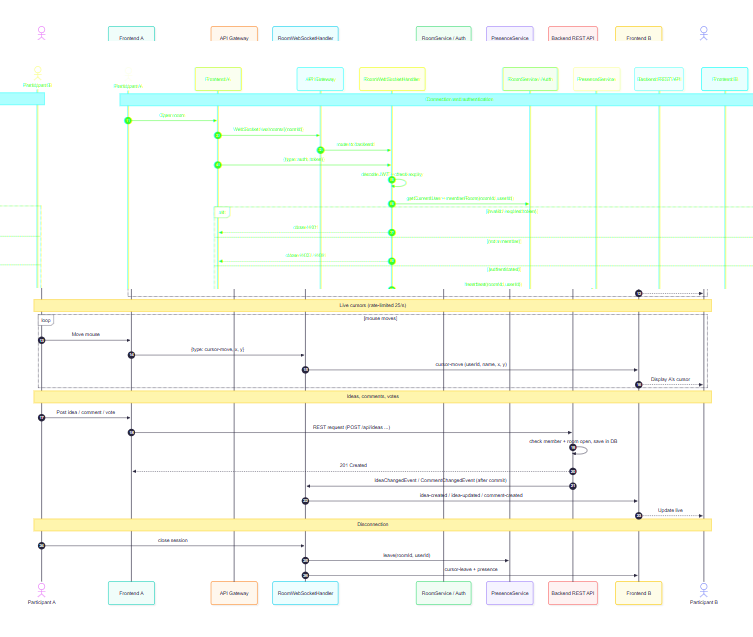
\includegraphics[width=0.95\textwidth]{images/sequence_diagram_1_realtime.png}
    \caption{Sequence Diagram — Authenticated WebSocket Channel, Presence, Throttled Cursors, and Transaction-Safe Live Updates.}
    \label{fig:sprint2-seq-realtime}
\end{figure}

Figure~\ref{fig:sprint2-seq-ai} details the AI idea generation and expansion pipeline (\texttt{US-42}--\texttt{US-44}). Upon receiving a topic or idea improvement request, \texttt{IdeaAIController} delegates to \texttt{AIOrchestrator}, which reserves user quota via \texttt{QuotaService} and invokes \texttt{ModelRouter}. Both failure branches—daily quota exhaustion (\texttt{DailyLimitReached}) and upstream LLM errors with automatic fallback and quota refund—are modeled alongside nominal JSON validation, database persistence via \texttt{Backend IdeaController}, and live room broadcasting.

\begin{figure}[htbp]
    \centering
    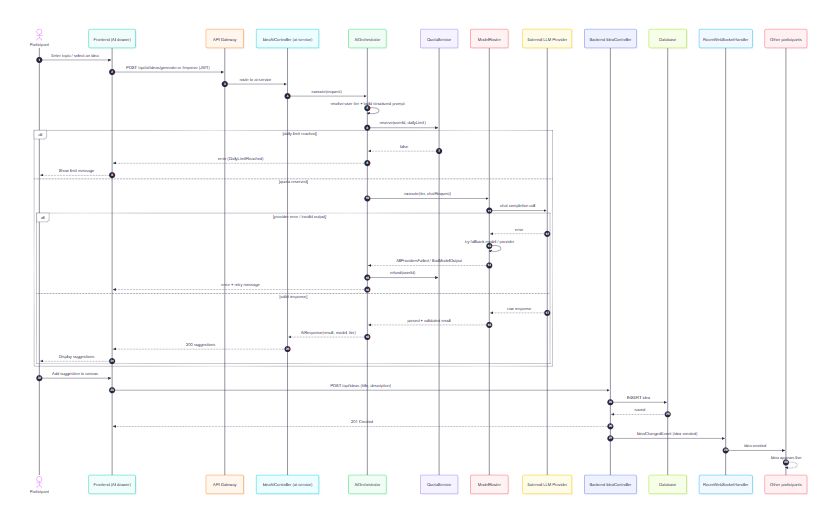
\includegraphics[width=0.98\textwidth]{images/sequence_diagram_2_ai.png}
    \caption{Sequence Diagram — AI Idea Generation and Improvement Pipeline with Quota Reservation and Fallback Handling.}
    \label{fig:sprint2-seq-ai}
\end{figure}

\subsection{State-Transition Diagram}

Figure~\ref{fig:sprint2-state} models the lifecycle of a brainstorming room controlled by the room creator (\texttt{US-16}, \texttt{US-17}). Upon creation, a room enters the \texttt{Open} state, allowing members to join via invitation code and add ideas, comments, and votes. Closing the room (\texttt{US-16}) transitions it to the \texttt{Closed} state, where new members, ideas, comments, and votes are blocked. A closed room can be \texttt{Reopened} to return to the \texttt{Open} state, or transition permanently to the terminal \texttt{Deleted} state (\texttt{US-17}) from either \texttt{Open} or \texttt{Closed}.

\begin{figure}[htbp]
    \centering
    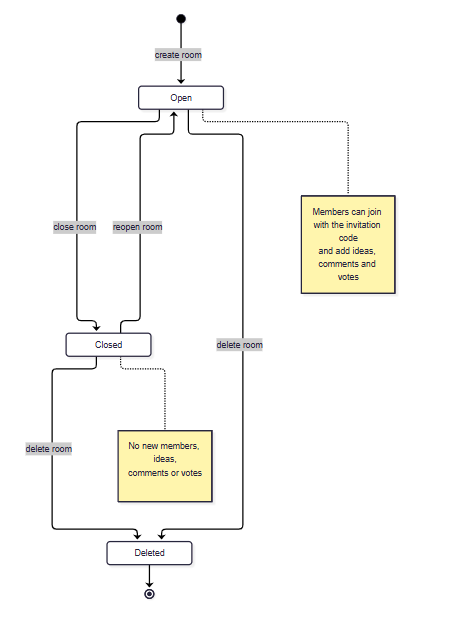
\includegraphics[width=0.52\textwidth]{images/state_diagram_room_lifecycle.png}
    \caption{State-Transition Diagram — Brainstorming Room Lifecycle (\texttt{Open}, \texttt{Closed}, \texttt{Deleted}).}
    \label{fig:sprint2-state}
\end{figure}

\section{Implementation}

During the implementation phase of Sprint 2, all 21 user stories were integrated across the Angular frontend, the Spring Boot core services, the WebSocket transport layer, and the \texttt{ai-service} microservice \cite{backlog}:
\begin{itemize}
    \item \textbf{Real-Time Synchronization Engine:} Authenticated WebSocket channels per room (\texttt{US-38}) stream committed domain mutations (\texttt{IdeaChangedEvent}, \texttt{CommentChangedEvent}) via \texttt{@TransactionalEventListener(phase = AFTER\_COMMIT)} (\texttt{US-39}), maintain live participant rosters via \texttt{PresenceService} heartbeats (\texttt{US-40}), and render normalized virtual cursor coordinates (\texttt{US-41}) \cite{backlog}.
    \item \textbf{Threaded Comments and Idea Organization:} Implemented comment creation (\texttt{US-32}), author edit/delete actions (\texttt{US-33}), and nested comment replies (\texttt{US-34}), alongside category CRUD (\texttt{US-27}, \texttt{US-28}), keyword search (\texttt{US-29}), and multi-criteria filtering and sorting (\texttt{US-30}) \cite{backlog}.
    \item \textbf{Room Governance, AI Core, and Demo Reset:} Delivered creator controls to edit room details (\texttt{US-13}), preview/remove participants (\texttt{US-14}, \texttt{US-15}), and close or delete rooms (\texttt{US-16}, \texttt{US-17}); implemented \texttt{AIOrchestrator} and \texttt{ModelRouter} (\texttt{US-42}) supporting topic-based generation (\texttt{US-43}) and idea expansion (\texttt{US-44}); added profile name/avatar editing (\texttt{US-5}); and provided a deterministic demo reset mechanism (\texttt{T5}) \cite{backlog}.
\end{itemize}

Figures~\ref{fig:ui-cursors} through \ref{fig:ui-ai} reserve the exact layout slots for the Sprint 2 user interface captures, styled using the same framed diagram placeholder convention as Chapter~2.

\begin{figure}[htbp]
    \centering
    \begin{screenshotplaceholder}
        \texttt{\bfseries\color{mindNavy} [fig-ui-live-cursors]}\\[4pt]
        \small\textit{\color{mindSlate}(Insert screenshot file: \texttt{fig-ui-live-cursors.png} — Online Presence Bar \& Live Cursors)}
    \end{screenshotplaceholder}
    \caption{Live Room Workspace Showing Online Presence Bar (\texttt{US-40}) and Real-Time Participant Cursors (\texttt{US-41}).}
    \label{fig:ui-cursors}
\end{figure}

\begin{figure}[htbp]
    \centering
    \begin{screenshotplaceholder}
        \texttt{\bfseries\color{mindNavy} [fig-ui-threaded-comments]}\\[4pt]
        \small\textit{\color{mindSlate}(Insert screenshot file: \texttt{fig-ui-threaded-comments.png} — Idea Card Comments, Edit/Delete \& Replies)}
    \end{screenshotplaceholder}
    \caption{Idea Card with Threaded Comments, Edit/Delete Controls, and Nested Replies (\texttt{US-32}, \texttt{US-33}, \texttt{US-34}).}
    \label{fig:ui-comments}
\end{figure}

\begin{figure}[htbp]
    \centering
    \begin{screenshotplaceholder}
        \texttt{\bfseries\color{mindNavy} [fig-ui-categories-filters]}\\[4pt]
        \small\textit{\color{mindSlate}(Insert screenshot file: \texttt{fig-ui-categories-filters.png} — Categories Modal \& Search/Filter/Sort Toolbar)}
    \end{screenshotplaceholder}
    \caption{Category Management Modal and Multi-Criteria Search, Filter, and Sort Toolbar (\texttt{US-27}--\texttt{US-30}).}
    \label{fig:ui-categories}
\end{figure}

\begin{figure}[htbp]
    \centering
    \begin{screenshotplaceholder}
        \texttt{\bfseries\color{mindNavy} [fig-ui-room-governance]}\\[4pt]
        \small\textit{\color{mindSlate}(Insert screenshot file: \texttt{fig-ui-room-governance.png} — Room Creator Settings, Participants \& Close/Delete)}
    \end{screenshotplaceholder}
    \caption{Room Creator Settings Panel — Edit Details, Manage Participants, and Close/Delete Room (\texttt{US-13}--\texttt{US-17}).}
    \label{fig:ui-room-settings}
\end{figure}

\begin{figure}[htbp]
    \centering
    \begin{screenshotplaceholder}
        \texttt{\bfseries\color{mindNavy} [fig-ui-ai-assistant]}\\[4pt]
        \small\textit{\color{mindSlate}(Insert screenshot file: \texttt{fig-ui-ai-assistant.png} — AI Topic Idea Generation \& Idea Expansion Modal)}
    \end{screenshotplaceholder}
    \caption{AI Ideation Assistant — Topic-Based Idea Generation (\texttt{US-43}) and Idea Expansion Modal (\texttt{US-44}).}
    \label{fig:ui-ai}
\end{figure}

\section{Sprint Review and Sprint Retrospective}

\subsection{Sprint Review}

At the conclusion of Sprint 2, all \textbf{21 planned user stories} were demonstrated and validated on the shared staging environment \cite{backlog}. Multi-browser testing confirmed instantaneous synchronization of newly posted ideas, votes, threaded comments, active presence rosters, and normalized participant cursors. Furthermore, category organization, keyword search, multi-criteria filtering and sorting, room creator moderation controls, profile customization, deterministic demo reset, and AI-assisted idea generation and expansion were verified and accepted.

\subsection{Sprint Retrospective}

\begin{itemize}
    \item \textbf{What Went Well:} Isolating external LLM calls inside \texttt{AIOrchestrator} and \texttt{ModelRouter} (\texttt{US-42}) kept prompt formatting, JSON schema validation, fallback routing, and quota refunds cleanly separated from core room logic. Scoping WebSocket subscriptions per room (\texttt{US-38}) ensured strict event isolation and predictable state updates.
    \item \textbf{What Could Be Improved:} Unthrottled pointer tracking initially generated excessive WebSocket frame volume; enforcing client-side throttling ($25\text{ events/s}$) eliminated network congestion while preserving smooth cursor interpolation. Additionally, SaaS subscription tiers, advanced AI analytical tools, session exports, and administrative dashboards remained scheduled for Sprint 3.
    \item \textbf{Action Items for Sprint 3:} Implement subscription plans and quota enforcement (\texttt{US-54}--\texttt{US-59}), expand the \texttt{ai-service} capabilities (semantic clustering, session summarization, action plan generation, risk detection, and idea comparison), add session export and admin governance portals, and execute automated end-to-end tests (\texttt{T6}) and production security hardening (\texttt{T7}) \cite{backlog}.
\end{itemize}

\section{Conclusion}

Sprint 2 transformed \textbf{MindSpark} from a foundational ideation prototype into a responsive, real-time collaborative workspace augmented by generative AI \cite{backlog}. With authenticated room channels, live presence and cursors, threaded discussions, structured categorization, room governance, and AI-powered idea generation and expansion operational, the platform is prepared for \textbf{Sprint 3}, which focuses on SaaS monetization, advanced AI synthesis, platform administration, and production hardening \cite{backlog}.
